\documentclass[11pt,a4paper]{article}
\usepackage{fontspec}
\usepackage[french]{babel}
\usepackage[margin=2cm]{geometry}
\usepackage{amsmath,amssymb}
\usepackage{booktabs,tabularx,array}
\usepackage{enumitem}
\usepackage{xcolor}
\usepackage{graphicx}
\usepackage[most]{tcolorbox}
\usepackage{titlesec}
\usepackage[hidelinks]{hyperref}

\definecolor{bleu}{HTML}{1F5FA8}
\definecolor{orange}{HTML}{D9822B}
\definecolor{rouge}{HTML}{C0392B}
\definecolor{vert}{HTML}{2E8B57}
\definecolor{gris}{HTML}{6B7079}

\setlist{itemsep=2pt,topsep=3pt,leftmargin=1.4em}
\setlength{\parskip}{5pt}
\setlength{\parindent}{0pt}
\titleformat{\section}{\Large\bfseries\color{bleu}}{\thesection.}{0.5em}{}
\titleformat{\subsection}{\large\bfseries\color{bleu!80!black}}{\thesubsection}{0.5em}{}
\titlespacing*{\section}{0pt}{14pt}{4pt}
\titlespacing*{\subsection}{0pt}{10pt}{2pt}

\newtcolorbox{cadre}[1]{colback=bleu!5,colframe=bleu,boxrule=0.6pt,arc=2pt,
  left=6pt,right=6pt,top=4pt,bottom=4pt,fonttitle=\bfseries,title={#1}}
\newtcolorbox{prof}[1]{colback=gris!7,colframe=gris,boxrule=0.6pt,arc=2pt,
  left=6pt,right=6pt,top=4pt,bottom=4pt,fonttitle=\bfseries,title={#1}}
\newtcolorbox{intuition}{colback=orange!7,colframe=orange,boxrule=0.6pt,arc=2pt,
  left=6pt,right=6pt,top=4pt,bottom=4pt,fonttitle=\bfseries,title={Intuition}}
\newtcolorbox{attention}{colback=rouge!5,colframe=rouge,boxrule=0.6pt,arc=2pt,
  left=6pt,right=6pt,top=4pt,bottom=4pt,fonttitle=\bfseries,title={Attention}}
\newcommand{\f}[1]{\texttt{#1}}
\newcommand{\en}[1]{\textit{«~#1~»}}

\begin{document}

\begin{center}
{\LARGE\bfseries Projet SMA : températures extrêmes à Brest}\\[4pt]
{\large Tout le projet expliqué pas à pas : le sujet du prof, ce qu'on rend, la méthode, les résultats}\\[4pt]
{\small\color{gris} IMT Atlantique, TAF MCE -- « Stochastic Processes for Environmental Data » (Pierre Tandeo), 2026}
\end{center}

\begin{cadre}{L'essentiel en 6 lignes}
\begin{itemize}
  \item \textbf{Ce qu'on rend :} \textbf{un seul notebook Jupyter par groupe}, celui du prof complété (les cellules \f{\#\#\# TO DO \#\#\#}), déposé sur \textbf{Moodle} avant le \textbf{vendredi 30 octobre 2026}.
  \item \textbf{Partie 1 (statistiques) :} le cycle saisonnier des températures à Brest, puis les vagues de chaleur (durée, intensité).
  \item \textbf{Partie 2 (machine learning) :} prédire la température maximale de chaque année jusqu'en 2100 sous 3 scénarios de CO2, \textbf{sous forme de probabilités}, et répondre : \en{quelle probabilité de dépasser 40\,°C à Brest d'ici 2100 ?} Puis refaire pour les minimales.
  \item \textbf{C'est fait :} le notebook complet est \f{rendu/miniprojet\_MCE\_SMA\_2026\_groupe.ipynb}. Il tourne en 15 secondes et donne toujours les mêmes chiffres.
  \item \textbf{Il reste :} mettre les noms du groupe, le relancer sur Colab, le relire, le déposer (section~\ref{sec:reste}).
\end{itemize}
\end{cadre}

{\setcounter{tocdepth}{1}\tableofcontents}
\newpage

%======================================================================
\section{Le sujet, exactement comme le prof l'a donné}

\subsection{Les sources du prof}

Tout ce qui vient du prof est dans le dossier \f{projet-sma/sujet\_prof/} :

\begin{tabularx}{\linewidth}{@{}lX@{}}
\toprule
\textbf{Fichier} & \textbf{Ce que c'est} \\
\midrule
\f{Projet SMA Stochastic Processes 2026.pdf} & Les slides de présentation du mini-projet (Pierre Tandeo, \f{pierre.tandeo@imt-atlantique.fr}) : objectifs, données, scénarios, méthodes, notation, date limite. \\
\f{miniprojet\_MCE\_SMA\_2026\_students.ipynb} & \textbf{Le notebook à compléter.} Il contient les consignes de chaque question et des cellules \f{\#\#\# TO DO \#\#\#} vides. \\
\f{data/daily\_temp\_brest.csv} & Température \textbf{moyenne de chaque jour} à Brest, du 1\textsuperscript{er} janvier 1940 au 31 décembre 2025 (31\,412 jours), en °C. \\
\f{data/yearly\_temp\_brest.csv} & Pour chaque année 1940--2025 : température \textbf{maximale} et \textbf{minimale} de l'année (°C), et CO2 mondial (ppm). \\
\f{data/yearly\_future\_co2.csv} & CO2 de 2026 à 2100 sous les 3 scénarios SSP1-2.6, SSP2-4.5, SSP5-8.5 (ppm). \\
\f{Compte Rendu Projet Processus Gaussiens 2026.ppsx} & Les slides du cours sur les processus gaussiens (loi normale, théorème central limite, vecteurs gaussiens, processus de Wiener). Ce n'est pas le sujet, mais c'est le cours sur lequel s'appuie le projet. \\
\bottomrule
\end{tabularx}

\subsection{Ce que disent les slides}

\begin{prof}{Slides du prof -- objectifs (texte original)}
\textbf{Final objective:} predict time series in the future; create an ensemble of artificial forecasts.\\
\textbf{Stochastic modeling:} use recent neural networks (e.g., diffusion models); condition it to an external variable (CO2).\\
\textbf{AI-driven approach:} code it using PyTorch and GPU; let AI help you.\\
\textbf{Climate application:} real environmental data (temperatures); compute statistics of extremes in the future.
\end{prof}

Traduction : on veut \textbf{prédire le futur}, mais pas avec une seule valeur : avec un \textbf{ensemble de prévisions artificielles} (plein de futurs possibles), \textbf{conditionné au CO2}, codé en \textbf{PyTorch}, pour calculer des \textbf{statistiques d'extrêmes}.

\begin{prof}{Slides du prof -- les deux parties (texte original)}
\textbf{Part 1: Statistical analysis.} Seasonal cycle: distribution of the daily temperature over a typical year, extract the 90\% quantile. Intensity-duration plot: identify extreme events (heat waves) exceeding the 90\% quantile during several consecutive days.\\[3pt]
\textbf{Part 2: Machine learning.} Probabilistic forecasts: make probabilistic predictions in the future, use Monte-Carlo or parametric methods, condition your forecasts on CO2 emissions. Question and additional study: what is the probability to exceed 40°C in Brest, at the horizon 2100? Make the same analysis with the minimum annual temperatures.
\end{prof}

\subsection{Comment le prof note}

\begin{prof}{Slides du prof -- « Evaluation of this mini-project » (texte original)}
\textbf{Quality of the code:} must be concise; comments are welcome.\\
\textbf{Quality of the outputs:} you are dealing with physical variables; do not forget the units (e.g., °C, ppm).\\
\textbf{Explanation of the method:} you must describe mathematically the chosen approach; write it directly into the notebook using Latex.\\
\textbf{Discuss your results:} results have physical meaning; you should be able to comment the outputs.
\end{prof}

Donc 4 critères : un code \textbf{court et commenté}, des figures et chiffres \textbf{avec unités}, la méthode \textbf{écrite en maths (LaTeX) dans le notebook}, et des \textbf{commentaires physiques} sur chaque résultat. Le notebook rendu a été construit pour cocher ces 4 cases : chaque figure a des axes avec unités, chaque résultat est suivi d'une cellule « Comment », et la méthode est démontrée en LaTeX.

\subsection{Organisation pratique (slides)}
\begin{itemize}
  \item Télécharger le notebook et les trois jeux de données (liens Moodle dans les slides).
  \item \en{Use Google Colab to share the notebook with your five colleagues} : groupes de 5 ou 6.
  \item \en{Upload one notebook per group to Moodle} -- \textbf{Deadline: Friday, October 30, 2026}.
\end{itemize}

%======================================================================
\section{Faut-il remplir des notebooks ? Oui : voici exactement quoi}

On rend \textbf{le notebook du prof}, complété. Il y a \textbf{8 cellules \f{\#\#\# TO DO \#\#\#}}. Voici la consigne exacte de chacune (en anglais, comme dans le notebook) et ce qu'on y a mis.

\renewcommand{\arraystretch}{1.25}
\begin{tabularx}{\linewidth}{@{}c>{\raggedright\arraybackslash}X>{\raggedright\arraybackslash}p{5.6cm}@{}}
\toprule
\textbf{n°} & \textbf{Consigne du prof (verbatim)} & \textbf{Ce qu'on a fait} \\
\midrule
1 & \small\en{Compute the seasonal cycle of the mean temperature in Brest. To do so, for each day of the year (between 1 and 365), compute the quantiles at 10\%, 50\%, and 90\%. Apply a 1-month rolling mean to smooth the data. Plot the corresponding curves and comment on this figure.} & \small Quantiles par jour de l'année, lissage circulaire de 31 jours, figure + commentaire. (§\ref{sec:p1}) \\
2 & \small\en{Compute the duration and intensity of the different heat waves during the period 1940 to 2025. The duration corresponds to the number of consecutive days exceeding the 90\% quantile. The intensity is defined as the mean temperature anomaly during those consecutive days.} & \small Détection des vagues ($\ge 3$ jours), tableau des plus longues et plus intenses. \\
3 & \small\en{Make the following scatter plot of the heat waves in Brest, with: x-axis representing duration, y-axis representing intensity, and the color representing the year of appearance. Comment on this figure.} & \small Nuage de points + nombre de vagues par décennie. \\
4 & \small\en{Plot and comment on the maximum annual temperature in Brest from 1940 to 2025.} & \small Courbe + moyenne glissante 11 ans. (§\ref{sec:p2}) \\
5 & \small\en{Compute the correlation between the maximum annual temperature in Brest and the global annual CO2. To increase the linear correlation coefficient, test several transformations of those two variables.} & \small Tableau des corrélations (log, moyennes glissantes 5, 11, 21 ans). \\
6 & \small\en{Use recent machine learning methods to provide probabilistic predictions (not deterministic) of maximum annual temperatures until 2100, conditionally on the three main climate scenarios. [...] Do not forget to present your approach mathematically and to justify your choice.} & \small Modèle GEV conditionné au CO2, entraîné en PyTorch, bootstrap + Monte-Carlo ; maths en LaTeX ; validation. (§\ref{sec:methode}) \\
7 & \small\en{Based on your probabilistic predictions, provide the distribution of the maximum annual temperature in 2100 for the three climate scenarios (SSPs). [...] what is the probability of exceeding 40°C in Brest, by 2100, for the three climate scenarios?} & \small Histogrammes 2100 + tableau des probabilités. (§\ref{sec:40}) \\
8 & \small\en{Make the same study for the minimum annual temperatures in Brest. You can try a different approach to generate your predictions (without including the mathematical formulation).} & \small Autre approche (bootstrap des résidus), probabilité de gel. (§\ref{sec:min}) \\
\bottomrule
\end{tabularx}

On a aussi : remplacé la cellule d'import \f{\%pylab inline} (obsolète) par des imports explicites (\f{numpy}, \f{matplotlib}, \f{pandas}, \f{torch}) et fixé les graines aléatoires ; ajouté une conclusion à la fin. Toutes les autres cellules du prof sont gardées telles quelles.

%======================================================================
\section{Les données, expliquées}

\textbf{ERA5.} Les températures ne viennent pas d'un thermomètre, mais de la \textbf{réanalyse ERA5} du centre européen ECMWF : une reconstruction de l'atmosphère passée qui combine un modèle météo et toutes les observations disponibles, sur une grille d'environ 9\,km. La valeur « Brest » est celle d'une case de 9\,km, en partie sur la mer. Conséquence importante pour la discussion : \textbf{ERA5 lisse les pics}. Un thermomètre en ville peut monter plusieurs degrés plus haut que la case ERA5.

\textbf{Trois variables de température, à ne pas confondre :}
\begin{itemize}
  \item la \textbf{moyenne journalière} (partie 1) : la moyenne sur 24\,h d'un jour (nuit comprise) ;
  \item le \textbf{maximum annuel} (partie 2) : la température la plus haute atteinte dans l'année, souvent un après-midi de canicule. Ce n'est \emph{pas} le maximum des moyennes journalières, qui est plus bas ;
  \item le \textbf{minimum annuel} : la température la plus basse de l'année.
\end{itemize}

\textbf{CO2 et ppm.} ppm = parties par million : 400\,ppm veut dire 400 molécules de CO2 pour un million de molécules d'air. Le CO2 passe de 310\,ppm (1940) à 428\,ppm (2025).

\textbf{Les scénarios SSP} (\emph{Shared Socioeconomic Pathways}) sont les futurs possibles utilisés par le GIEC. Le nombre après le tiret est le forçage radiatif en 2100 (en W/m², le surplus d'énergie reçu par la Terre), pas du CO2 :

\begin{center}
\begin{tabular}{@{}llr@{}}
\toprule
\textbf{Scénario} & \textbf{Monde} & \textbf{CO2 en 2100} \\
\midrule
SSP1-2.6 & sobre : les émissions baissent vite & 400\,ppm \\
SSP2-4.5 & intermédiaire & 527\,ppm \\
SSP5-8.5 & très fossile & 946\,ppm \\
\bottomrule
\end{tabular}
\end{center}

%======================================================================
\section{Partie 1 : le passé, avec des statistiques}\label{sec:p1}

\subsection{Le cycle saisonnier}

\begin{intuition}
Un \textbf{quantile à 90\,\%} d'une liste de valeurs, c'est la valeur sous laquelle se trouvent 90\,\% d'entre elles. Pour le 15 juillet, on a 86 températures (une par année de 1940 à 2025) : le quantile à 90\,\% est la température que seuls les 10\,\% des 15 juillet les plus chauds dépassent. Le quantile à 50\,\% est la \textbf{médiane}, la valeur « normale ».
\end{intuition}

\textbf{La méthode, étape par étape :}
\begin{enumerate}
  \item On numérote les jours de 1 à 365. Le sujet demande 365 jours : on \textbf{retire les 29 février} (22 jours sur 31\,412, sans effet).
  \item Pour chaque jour $j$, on calcule les quantiles à 10, 50 et 90\,\% des 86 valeurs : $q_{10}(j)$, $q_{50}(j)$, $q_{90}(j)$.
  \item Ces courbes sont bruitées (86 valeurs par jour, c'est peu). On les \textbf{lisse par une moyenne glissante d'un mois} (31 jours centrés). Astuce : le cycle est \textbf{périodique}, donc pour lisser le 1\textsuperscript{er} janvier on utilise aussi les derniers jours de décembre (lissage « circulaire »).
\end{enumerate}

\begin{center}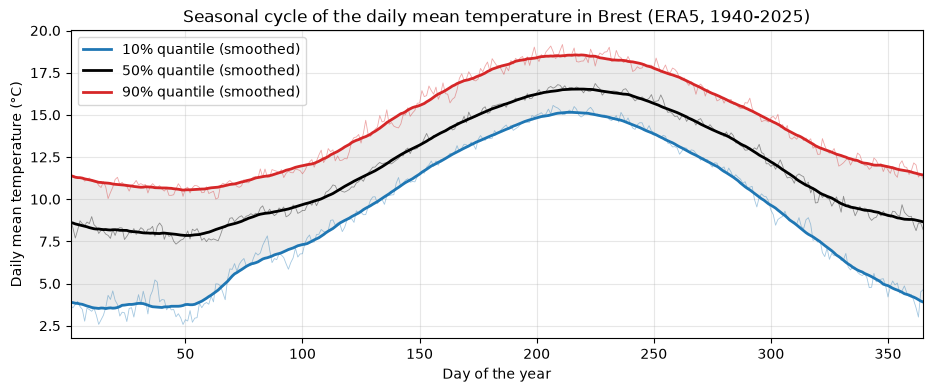
\includegraphics[width=\linewidth]{figures/cycle.png}\end{center}

\textbf{Ce qu'il faut en dire :}
\begin{itemize}
  \item Le minimum est fin février (médiane $\approx 7{,}8$\,°C), le maximum début août ($\approx 16{,}5$\,°C) : seulement $\approx 9$\,°C d'amplitude, et un retard d'environ 6 semaines sur le solstice. C'est la signature du \textbf{climat océanique} : l'océan stocke la chaleur l'été et la rend l'hiver.
  \item L'écart entre 10\,\% et 90\,\% est plus grand en hiver ($\approx 7$\,°C) qu'en été ($\approx 3{,}5$\,°C) : en hiver, tout dépend du vent (air océanique doux ou air continental froid).
  \item La courbe rouge (90\,\%) est le \textbf{seuil} qui sert à détecter les vagues de chaleur.
\end{itemize}

\subsection{Les vagues de chaleur}

\textbf{Définitions} (celles du prof, précisées) :
\begin{itemize}
  \item un jour est \textbf{chaud} si sa température dépasse le quantile à 90\,\% lissé \emph{de son jour de l'année} : $T_d > q_{90}(j_d)$ ;
  \item une \textbf{vague de chaleur} est une suite d'au moins \textbf{3 jours chauds consécutifs} (le prof dit \en{several consecutive days} ; 3 jours est la convention habituelle, c'est un choix à justifier) ;
  \item sa \textbf{durée} est son nombre de jours ;
  \item son \textbf{intensité} est l'anomalie moyenne pendant la vague, par rapport à la normale (la médiane lissée) :
\end{itemize}
\[
\text{intensité}=\frac{1}{|W|}\sum_{d\in W}\big(T_d-q_{50}(j_d)\big)\quad\text{en °C}.
\]

\textbf{Le résultat :} 421 vagues en 86 ans (environ 5 par an, logique : 10\,\% des jours sont « chauds »). Les plus longues : 14 jours (août 1955, août 1976, l'été de la grande sécheresse). La plus intense : \textbf{juillet 2022}, +7,7\,°C au-dessus de la normale pendant 3 jours.

\begin{center}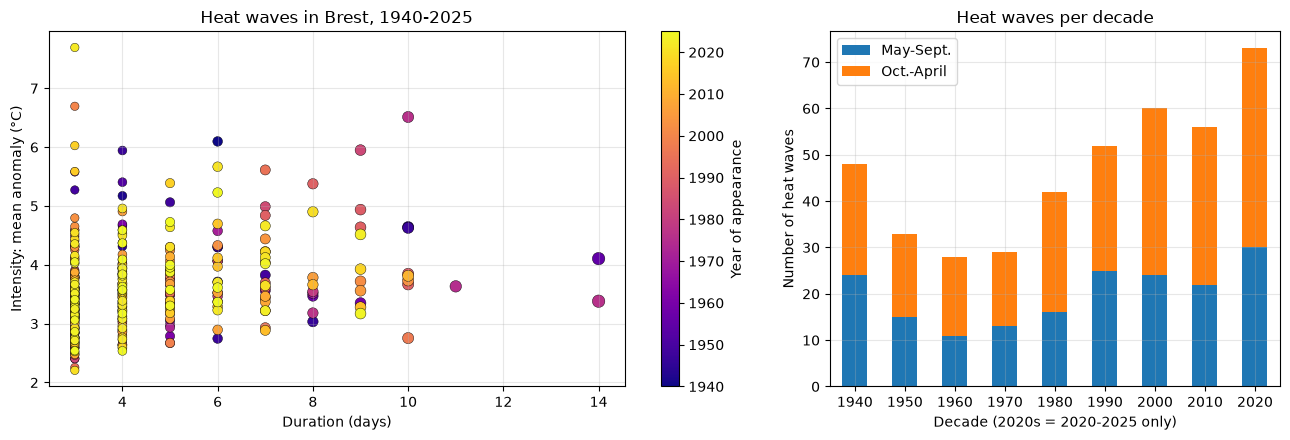
\includegraphics[width=\linewidth]{figures/vagues.png}\end{center}

\textbf{Ce qu'il faut en dire :}
\begin{itemize}
  \item La plupart des vagues sont courtes (3 à 5 jours) et d'intensité 2,5 à 5\,°C. Les plus intenses sont souvent courtes, et récentes (points jaunes en haut à gauche).
  \item Le signal le plus net est à droite : le \textbf{nombre} de vagues par décennie baisse jusqu'aux années 1960--70 puis \textbf{augmente fortement} : 73 vagues pour 2020--2025, qui ne comptent que 6 ans. C'est cohérent avec le réchauffement depuis les années 1980.
  \item Comme le seuil dépend du jour de l'année, la définition détecte aussi des épisodes \textbf{doux en hiver} (en orange) : ce sont des anomalies pour la saison, pas des journées chaudes dans l'absolu. Il faut le dire.
  \item \textbf{Limite :} les quantiles sont calculés sur toute la période 1940--2025. Dans un climat qui se réchauffe, le seuil est « trop bas » pour les années récentes, ce qui crée mécaniquement plus de vagues à la fin. C'est justement la tendance qu'on veut montrer, mais il faut en être conscient.
\end{itemize}

%======================================================================
\section{Partie 2 : le futur, avec du machine learning}\label{sec:p2}

\subsection{Le maximum annuel de 1940 à 2025}

\begin{center}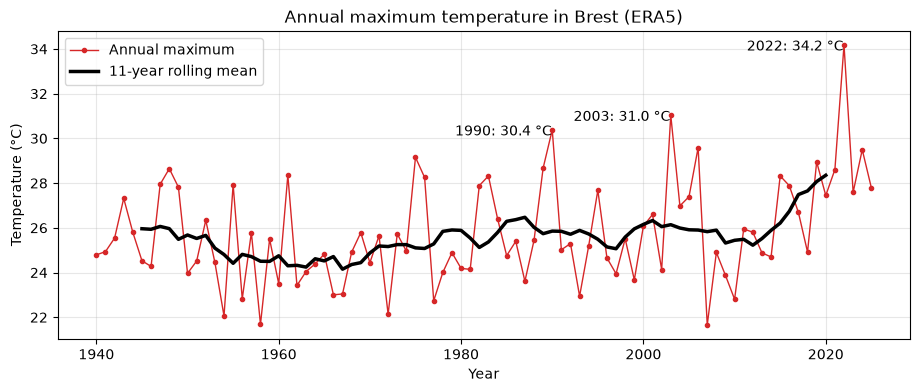
\includegraphics[width=\linewidth]{figures/tmax.png}\end{center}

Le maximum annuel saute beaucoup d'une année à l'autre (de 21,7 à 34,2\,°C), parce qu'il dépend de la météo de quelques jours. La moyenne glissante sur 11 ans est plate jusqu'aux années 1980 ($\approx 25$\,°C) puis monte d'environ 1,5 à 2\,°C. Moyenne 1940--1979 : 25,1\,°C ; 1980--2025 : 26,3\,°C. Le record est \textbf{2022 : 34,2\,°C}, loin devant 2003 (31,0\,°C).

\subsection{La corrélation avec le CO2}

\begin{intuition}
La \textbf{corrélation de Pearson} $r$ mesure à quel point deux variables sont alignées sur une droite : $r=1$ parfaitement alignées, $r=0$ aucun lien linéaire. $r = \dfrac{\mathrm{cov}(X,Y)}{\sigma_X\,\sigma_Y}$.
\end{intuition}

\begin{center}
\begin{tabular}{@{}lccc@{}}
\toprule
\textbf{Température \textbackslash{} CO2} & CO2 & $\ln$(CO2) & $\ln$(CO2/280) \\
\midrule
$T$ brute & 0,31 & 0,30 & 0,30 \\
$T$, moyenne glissante 5 ans & 0,49 & 0,47 & 0,47 \\
$T$, moyenne glissante 11 ans & 0,61 & 0,60 & 0,60 \\
$T$, moyenne glissante 21 ans & \textbf{0,83} & 0,82 & 0,82 \\
\bottomrule
\end{tabular}
\end{center}

\textbf{Comment l'expliquer :}
\begin{itemize}
  \item Brute, la corrélation est faible ($0{,}31$) : une année donnée, la \textbf{météo domine} le signal climatique.
  \item Le \textbf{log} ne change presque rien : entre 310 et 428\,ppm, $\ln$ est presque une droite. Et $\ln(C/280)=\ln C - \ln 280$ donne exactement le même $r$ que $\ln C$, car la corrélation ne change pas quand on ajoute une constante.
  \item La \textbf{moyenne glissante} enlève le bruit d'une année sur l'autre : $r$ monte à 0,83. Mais attention : ça ne veut pas dire qu'on sait prédire le maximum d'une année précise. Ça veut dire que le \textbf{niveau moyen} des extrêmes suit le CO2, avec beaucoup de hasard autour. C'est exactement pour ça qu'il faut une prévision \textbf{probabiliste}.
  \item On garde quand même $\ln$(CO2) dans le modèle, pour une raison physique : l'effet de serre du CO2 est \textbf{logarithmique} (forçage $\Delta F\approx 5{,}35\,\ln(C/C_0)$\,W/m²). Ça compte quand on extrapole jusqu'à 946\,ppm.
\end{itemize}

\subsection{La méthode : un modèle GEV appris en PyTorch, avec Monte-Carlo}\label{sec:methode}

\subsubsection*{Prévision probabiliste : l'idée}
Une prévision \emph{déterministe} dirait « en 2100, il fera 31\,°C ». Une prévision \emph{probabiliste} dit « en 2100, le maximum sera entre 26 et 37\,°C avec 90\,\% de chances ». On la représente par un \textbf{ensemble} : 10\,000 futurs possibles, tirés au hasard. Toute probabilité devient alors un comptage : « la proportion des 10\,000 futurs où l'on dépasse 40\,°C ». C'est la méthode de \textbf{Monte-Carlo} demandée par le prof.

\subsubsection*{Pourquoi la loi GEV}
Le cours (slides « Gaussian processes ») présente le \textbf{théorème central limite} : une \emph{somme} de nombreuses variables aléatoires tend vers une loi normale. Il existe l'équivalent pour un \emph{maximum} : le \textbf{théorème de Fisher--Tippett--Gnedenko}. Le maximum de nombreuses variables ne peut tendre que vers une seule famille de lois : la loi \textbf{GEV} (\emph{Generalised Extreme Value}). Or le maximum annuel est le maximum de 365 jours. La GEV est donc le choix naturel :
\[
F(t;\mu,\sigma,\xi)=\mathbb P(T\le t)=\exp\left\{-\left[1+\xi\,\frac{t-\mu}{\sigma}\right]^{-1/\xi}\right\}.
\]
Trois paramètres : la \textbf{position} $\mu$ (°C, où se situe la loi), l'\textbf{échelle} $\sigma$ (°C, sa largeur) et la \textbf{forme} $\xi$ (sans unité, la queue). Pour les températures, $\xi<0$ : la loi a une \textbf{borne supérieure} $\mu-\sigma/\xi$ (l'atmosphère ne peut pas chauffer à l'infini).

\subsubsection*{Conditionner au CO2}
Le climat change, donc la position dépend du CO2 de l'année :
\[
T_t \mid C_t \sim \mathrm{GEV}(\mu_t,\sigma,\xi),\qquad \mu_t=\beta_0+\beta_1\,\ln(C_t/C_0),\qquad C_0=280\ \text{ppm (pré-industriel)}.
\]
$\beta_1$ est la sensibilité du jour le plus chaud de Brest au CO2.

\subsubsection*{L'apprentissage en PyTorch}
On cherche les paramètres qui rendent les 86 années observées les plus probables : c'est le \textbf{maximum de vraisemblance}. On minimise la log-vraisemblance négative
\[
\mathcal L(\theta)=\sum_t\left[\log\sigma+\Big(1+\tfrac1\xi\Big)\log z_t+z_t^{-1/\xi}\right],\qquad z_t=1+\xi\,\frac{T_t-\mu_t}{\sigma},
\]
par \textbf{descente de gradient} (optimiseur Adam, PyTorch calcule les gradients automatiquement), exactement comme on entraîne un réseau de neurones. Deux contraintes physiques sont imposées à chaque pas : $\beta_1\ge 0$ (plus de CO2 ne refroidit pas) et $\xi\in[-0{,}5;-0{,}01]$ (queue bornée).

On a vérifié que PyTorch trouve le même optimum qu'un optimiseur classique (\f{scipy}) : $\beta_0=23{,}29$, $\beta_1=5{,}93$, $\log\sigma=0{,}644$, $\xi=-0{,}106$ dans les deux cas.

\subsubsection*{L'incertitude sur le modèle : le bootstrap}
86 années, c'est peu : les paramètres sont incertains, et cette incertitude grossit quand on extrapole à 946\,ppm. On entraîne donc \textbf{500 modèles en parallèle}, chacun sur un \textbf{échantillon bootstrap} des années (86 années tirées au hasard avec remise). La loi prédite est le \textbf{mélange} des 500 :
\[
p(T\mid C)\approx\frac1B\sum_{b=1}^{B}\mathrm{GEV}\Big(T;\ \beta_0^{(b)}+\beta_1^{(b)}\ln(C/C_0),\ \sigma^{(b)},\ \xi^{(b)}\Big),\qquad B=500.
\]

\subsubsection*{Le tirage Monte-Carlo}
Pour chaque scénario, 10\,000 trajectoires 2026--2100 : chaque trajectoire choisit un des 500 modèles au hasard, puis tire chaque année avec l'inverse de la fonction de répartition ($U$ uniforme sur $[0,1]$) :
\[
T=\mu+\frac{\sigma}{\xi}\Big[(-\ln U)^{-\xi}-1\Big].
\]

\subsubsection*{Pourquoi pas un modèle de diffusion ou un réseau de neurones ?}
Les slides citent les modèles de diffusion en exemple. Mais avec \textbf{86 points}, un réseau avec des milliers de paramètres surapprendrait, et rien ne garantit un comportement sensé à 946\,ppm, très loin des données. Notre modèle garde l'esprit du ML probabiliste moderne (PyTorch, entraînement par gradient, ensemble, échantillonnage) avec \textbf{4 paramètres qui ont un sens physique} et une forme justifiée par la théorie. C'est l'argument à donner au prof : \en{justify your choice}.

\subsection{La validation : est-ce que le modèle marche vraiment ?}

On fait comme si on était en 2000 : le modèle apprend sur \textbf{1940--2000} et prédit \textbf{2001--2025}, qu'il n'a jamais vues (avec un CO2 plus haut que tout ce qu'il connaît). On compare avec la vérité grâce au \textbf{CRPS} :
\[
\mathrm{CRPS}(F,y)=\int\big(F(u)-\mathbf 1\{u\ge y\}\big)^2\,du=\mathbb E|X-y|-\tfrac12\,\mathbb E|X-X'|.
\]
C'est l'erreur absolue généralisée à une loi : premier terme, la distance moyenne entre les tirages et la vraie valeur ; second terme, on retire l'étalement. En °C, plus bas = mieux.

\begin{center}
\begin{tabular}{@{}lc@{}}
\toprule
\textbf{Modèle (appris sur 1940--2000)} & \textbf{CRPS 2001--2025} \\
\midrule
Climat constant (1940--2000, sans tendance) & 1,82\,°C \\
Droite en $\ln$(CO2) + bruit gaussien (référence du groupe) & 1,70\,°C \\
\textbf{Notre GEV + bootstrap} & \textbf{1,66\,°C} \\
\bottomrule
\end{tabular}
\end{center}

Notre modèle fait mieux que les deux références. C'est aussi un score qui bat le modèle de référence de la compétition interne du groupe (1,70\,°C). Le gain sur le modèle gaussien est modeste : avec 25 années de test, deux bons modèles sont proches. Il faut le dire honnêtement.

Ensuite, pour les prévisions, le modèle est \textbf{ré-entraîné sur toutes les données 1940--2025}.

\subsection{Les projections jusqu'en 2100}

\begin{center}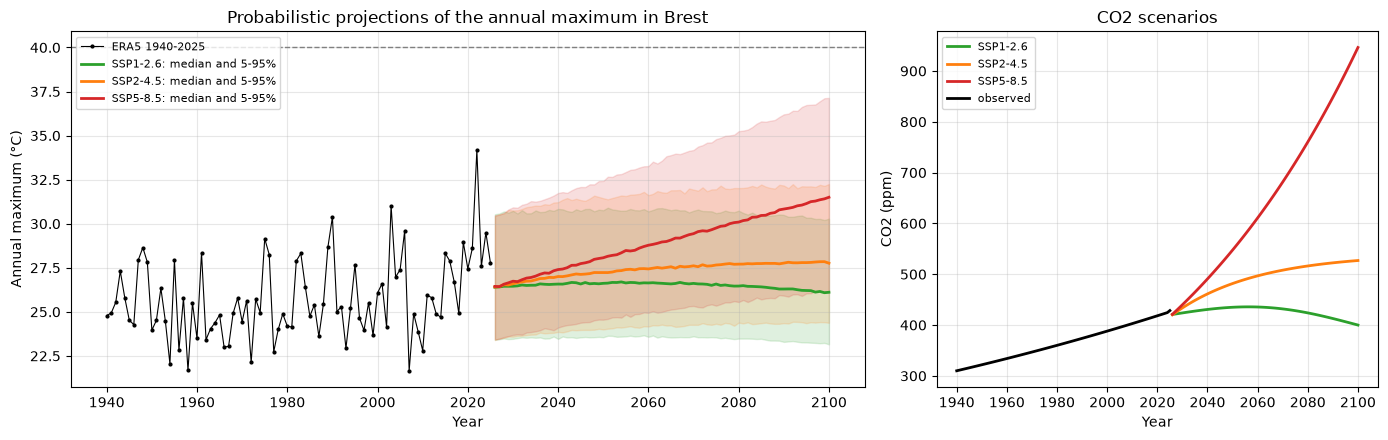
\includegraphics[width=\linewidth]{figures/projection_max.png}\end{center}

Les trois scénarios partent du même niveau en 2026 (médiane $\approx 26{,}5$\,°C) puis divergent après 2040. Médiane 2100 : $\approx 26{,}1$\,°C (SSP1-2.6, le CO2 redescend), $\approx 27{,}8$\,°C (SSP2-4.5), $\approx 31{,}5$\,°C (SSP5-8.5) : sous SSP5-8.5, une année « normale » de 2100 serait aussi chaude que les années les plus chaudes du XX\textsuperscript{e} siècle. La bande 5--95\,\% est large (la météo d'une année) et s'élargit sous SSP5-8.5, car l'incertitude sur $\beta_1$ est multipliée par une plus grande hausse du CO2.

\subsection{La réponse : la probabilité de dépasser 40\,°C}\label{sec:40}

\begin{center}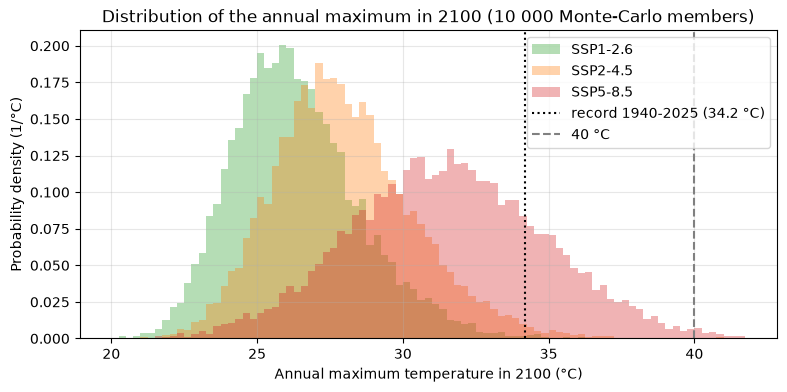
\includegraphics[width=0.85\linewidth]{figures/distribution_2100.png}\end{center}

\begin{attention}
La question \en{probability of exceeding 40°C in Brest, by 2100} peut se lire de \textbf{deux façons} : (a) la probabilité que \textbf{l'année 2100} dépasse 40\,°C ; (b) la probabilité qu'\textbf{au moins une année d'ici 2100} dépasse 40\,°C. (b) est bien plus grande. Le notebook donne les deux, en le disant clairement.
\end{attention}

\begin{center}
\begin{tabular}{@{}lcccc@{}}
\toprule
\textbf{Scénario} & \textbf{CO2 2100} & \textbf{Médiane 2100} & \textbf{(a) l'année 2100} & \textbf{(b) au moins 1 an} \\
 & & & \small $>40$\,°C & \small $>40$\,°C en 2026--2100 \\
\midrule
SSP1-2.6 & 400\,ppm & 26,1\,°C & $\approx 0{,}01$\,\% & $\approx 0{,}3$\,\% \\
SSP2-4.5 & 527\,ppm & 27,8\,°C & $\approx 0{,}02$\,\% & $\approx 0{,}7$\,\% \\
SSP5-8.5 & 946\,ppm & 31,5\,°C & $\approx 0{,}75$\,\% & $\approx 8$\,\% \\
\bottomrule
\end{tabular}
\end{center}

\textbf{Ce qu'il faut en dire :}
\begin{itemize}
  \item Dépasser 40\,°C une année donnée reste très improbable, même en 2100 sous le pire scénario ($<1$\,\%).
  \item Mais sur 75 ans, le risque \textbf{s'accumule} : sous SSP5-8.5, environ \textbf{1 chance sur 12} qu'au moins une année dépasse 40\,°C, contre moins de 1\,\% sous SSP1-2.6. Le scénario d'émissions multiplie ce risque par plus de 20.
  \item La borne supérieure de la GEV ($\approx 43$\,°C en SSP1-2.6, $\approx 50$\,°C en SSP5-8.5) dit que 40\,°C est possible, mais très loin dans la queue.
\end{itemize}

\textbf{Les limites à écrire (le prof note la discussion) :}
\begin{enumerate}
  \item \textbf{ERA5 lisse les pics} (case de 9\,km, en partie sur la mer) : une station météo à Brest peut être plusieurs degrés au-dessus. Nos probabilités concernent la variable ERA5 et \textbf{sous-estiment} le risque pour un thermomètre. (Par exemple, en juillet 2022, les stations bretonnes ont battu des records bien au-dessus des 34,2\,°C d'ERA5 ; si vous citez un chiffre de Météo-France, vérifiez-le à la source.)
  \item Le modèle ne connaît que le CO2 : il ignore les aérosols, les changements de circulation atmosphérique, la sécheresse des sols, qui amplifient les canicules.
  \item 946\,ppm est loin des données (310--428\,ppm) : c'est une \textbf{extrapolation}, en partie couverte par l'incertitude du bootstrap.
  \item Une probabilité de 0,01\,\% correspond à 1 tirage sur 10\,000 : ce sont des \textbf{ordres de grandeur}, pas des valeurs précises.
\end{enumerate}

\subsection{Les températures minimales}\label{sec:min}

Le prof autorise \en{a different approach [...] without including the mathematical formulation}. On a donc pris une approche \textbf{non paramétrique}, différente de la GEV :
\begin{itemize}
  \item une droite en $\ln$(CO2) ajustée par moindres carrés ;
  \item \textbf{aucune loi supposée pour le bruit} : chaque futur ajoute des résidus \textbf{tirés parmi les écarts réellement observés} (bootstrap des résidus) ;
  \item la droite est ré-ajustée sur 500 échantillons bootstrap des années, pour l'incertitude du modèle.
\end{itemize}

\begin{center}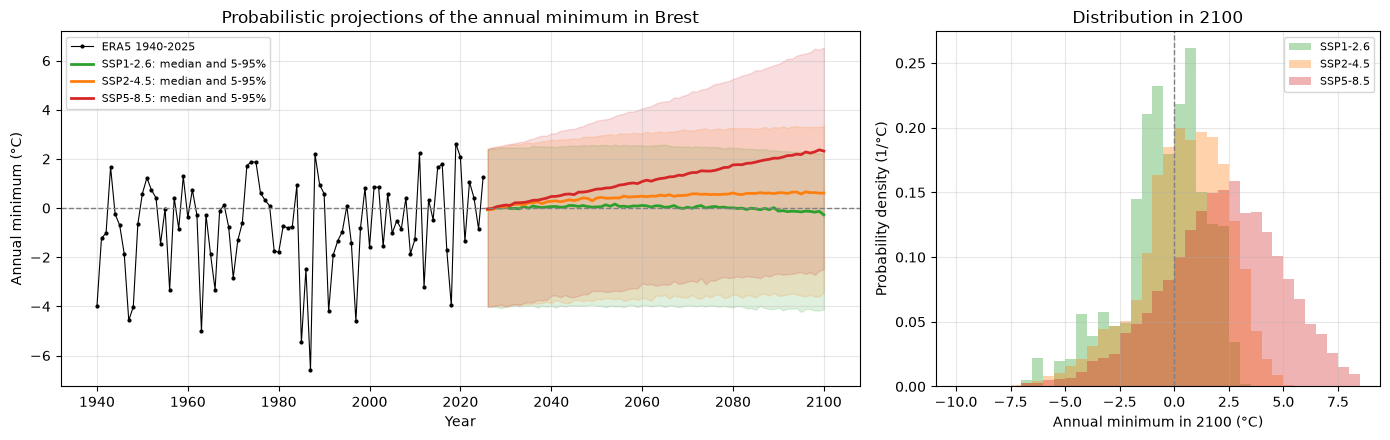
\includegraphics[width=\linewidth]{figures/projection_min.png}\end{center}

\textbf{Ce qu'il faut en dire :}
\begin{itemize}
  \item Le minimum est beaucoup moins lié au CO2 que le maximum ($r\approx 0{,}15$) : il dépend de rares coups de froid continentaux (1985, 1987 à $-6{,}6$\,°C).
  \item Validation (appris sur 1940--2000) : CRPS 1,09\,°C, proche du modèle gaussien (1,06\,°C). Les minima sont surtout de la météo, difficiles à prévoir. Honnêtement, cette approche ne fait pas mieux que la référence ; elle a l'avantage de ne rien supposer sur la forme de la loi.
  \item Médiane 2100 : $-0{,}3$\,°C (SSP1-2.6), $+0{,}6$\,°C (SSP2-4.5), $+2{,}3$\,°C (SSP5-8.5).
  \item \textbf{La question parallèle aux 40\,°C : le gel.} De 1940 à 2025, 60\,\% des années ont gelé (minimum $<0$\,°C). En 2100 : $\approx 54$\,\%, 38\,\% et 20\,\%. Sous SSP5-8.5, \textbf{4 années sur 5 n'auraient plus du tout de gel} à Brest (dans ERA5). Le gel ne disparaît pas pour autant : chaque trajectoire a au moins une année avec gel entre 2026 et 2100.
  \item Les histogrammes sont « en dents de scie » parce que le bruit est tiré parmi 86 résidus seulement.
\end{itemize}

%======================================================================
\section{Ce qu'il reste à faire avant le 30 octobre}\label{sec:reste}

\begin{cadre}{Check-list}
\begin{enumerate}
  \item \textbf{Mettre les noms} des 5 ou 6 membres dans la 2\textsuperscript{e} cellule (« The five students are... »).
  \item \textbf{Relancer sur Google Colab} : ouvrir \f{rendu/miniprojet\_MCE\_SMA\_2026\_groupe.ipynb} dans Colab, envoyer les 3 fichiers CSV (\f{daily\_temp\_brest.csv}, \f{yearly\_temp\_brest.csv}, \f{yearly\_future\_co2.csv}) avec le panneau « Fichiers », puis « Exécution > Tout exécuter ». Tout tourne sur CPU en quelques secondes ; pas besoin de GPU.
  \item \textbf{Relire les commentaires} et les ajuster à votre façon de parler (ils sont en anglais, comme le notebook du prof ; on peut les passer en français si le groupe préfère).
  \item \textbf{Vérifier les chiffres} : les valeurs écrites dans les commentaires correspondent aux sorties avec les graines fixées. Si vous changez du code, relisez les commentaires.
  \item \textbf{Déposer un seul notebook} pour le groupe sur Moodle.
\end{enumerate}
\end{cadre}

\textbf{Les choix qu'on a faits et qu'il faut savoir défendre à l'oral :}
\begin{itemize}
  \item 29 février retiré ; lissage de 31 jours circulaire ;
  \item vague = au moins 3 jours ; intensité mesurée par rapport à la médiane (la « normale ») ;
  \item covariable $\ln$(CO2/280) pour la physique du forçage ;
  \item GEV plutôt que réseau de neurones (86 points, extrapolation, théorie des extrêmes) ;
  \item contraintes $\beta_1\ge0$ et $\xi<0$, justifiées par la physique et pas par le score ;
  \item les deux lectures de la question des 40\,°C.
\end{itemize}

\textbf{Les fichiers, dans le dossier \f{projet-sma/rendu/} :}
\begin{itemize}
  \item \f{miniprojet\_MCE\_SMA\_2026\_groupe.ipynb} : \textbf{le notebook à rendre}, déjà exécuté (figures et chiffres visibles) ;
  \item les 3 fichiers \f{.csv} : les données du prof, à mettre à côté du notebook ;
  \item \f{build\_notebook.py} et \f{comments.py} : les scripts qui ont généré le notebook à partir de celui du prof (pas à rendre) ;
  \item \f{explication/} : ce document et sa source LaTeX.
\end{itemize}

%======================================================================
\section{Petit glossaire}

\begin{description}[leftmargin=0pt,itemsep=3pt]
  \item[Quantile à $p$\,\%] La valeur sous laquelle se trouvent $p$\,\% des données. Le quantile à 50\,\% est la médiane.
  \item[Anomalie] L'écart entre une température et la normale de son jour (ici la médiane lissée).
  \item[Prévision probabiliste] Une loi de probabilité (ou 10\,000 tirages) au lieu d'une seule valeur.
  \item[Monte-Carlo] Calculer une probabilité en tirant au hasard un grand nombre de scénarios et en comptant.
  \item[GEV] La loi des maxima (théorème de Fisher--Tippett--Gnedenko), l'équivalent de la loi normale pour les maximums.
  \item[Maximum de vraisemblance] Choisir les paramètres qui rendent les données observées les plus probables.
  \item[Bootstrap] Ré-échantillonner les données avec remise pour mesurer l'incertitude d'un modèle.
  \item[CRPS] Score d'une prévision probabiliste, en °C : l'erreur absolue généralisée à une loi. Plus bas = mieux.
  \item[SSP] Scénario socio-économique du GIEC ; le nombre est le forçage radiatif en 2100 (W/m²).
  \item[ERA5] Réanalyse de l'ECMWF : reconstruction de l'atmosphère passée sur une grille de $\approx 9$\,km.
\end{description}

\end{document}
